\documentclass{standalone}
\usepackage{tikz}
\usetikzlibrary{calc,positioning,shapes,decorations.pathmorphing}
\usetikzlibrary{hobby} % for blobs, see http://tex.stackexchange.com/a/145276

\def\gridopacity{100}
\def\gridopacity{0}

\begin{document}%
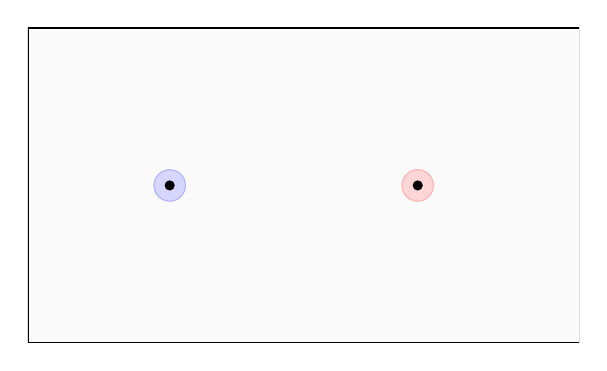
\begin{tikzpicture}
\tikzset{>=latex} % arrow heads
\draw[step=1,black!15,very thin,opacity=\gridopacity] (0,0) grid (5,4);


% blobs labeled a,b,c,d (in to out)

\ifdefined\arga
   \def\drawstartlabelb{}
   \def\drawdestlabelb{}
\fi

\ifdefined\argb
   \def\drawstartlabelc{}
   \def\drawdestlabelb{}
\fi

\ifdefined\argc
   \def\drawstartlabelc{}
   \def\drawdestc{}
   \def\drawdestlabelc{}
\fi

\ifdefined\argd
   \def\drawstartlabeld{}
   \def\drawdestc{}
   \def\drawdestlabelc{}
\fi

\ifdefined\arge
   \def\drawstartlabeld{}
   \def\drawdestc{}
   \def\drawdestd{}
   \def\drawdestlabeld{}
   \def\drawfvert{}
\fi

\ifdefined\argf
   \def\drawstartlabeld{}
   \def\drawdestc{}
   \def\drawdestd{}
   \def\drawdestlabeld{}
   \def\drawfvert{}
   \def\drawpatha{}
\fi

\ifdefined\argg
   \def\drawstartlabeld{}
   \def\drawdestc{}
   \def\drawdestd{}
   \def\drawdestlabeld{}
   \def\drawfvert{}
   \def\drawpatha{}
   \def\drawpathb{}
\fi

\begin{scope}
\clip (0,0) rectangle (7,4);
\fill[black!2] (0,0) rectangle (7,4);


% draw some contour blobs

% goal upnderneath
\ifdefined\drawdestd
\path[use Hobby shortcut,closed=true,fill=red!10]
   (4.8,3.5) .. (5.3,3.0) .. (6.3,2.0) .. (6.6,0.9) .. (4.8,0.5) .. (4.15,1.3) .. (2.93,3.0);
\fi



% start side
\ifdefined\drawstartlabelb
\path[draw,use Hobby shortcut,closed=true,fill=blue!14,densely dashed,draw=blue]
   (1.2,2.4) .. (1.5,2.6) .. (2.3,2.0) .. (2.2,1.3) .. (1.5,1.5);
\node[circle,fill=black!2,fill opacity=0.8,text opacity=1.0,inner sep=0.5pt,text=blue] at (1.4,2.6) {$D_s$};
\fi

\ifdefined\drawstartlabelc
\path[draw,use Hobby shortcut,closed=true,fill=blue!12,densely dashed,draw=blue]
   (1.4,3.1) .. (2.0,2.8) .. (2.8,2.0) .. (2.5,0.8) .. (1.5,1.0);
\path[draw,use Hobby shortcut,closed=true,fill=blue!14,draw=blue!28]
   (1.2,2.4) .. (1.5,2.6) .. (2.3,2.0) .. (2.2,1.3) .. (1.5,1.5);
\node[circle,fill=black!2,fill opacity=0.8,text opacity=1.0,inner sep=0.5pt,text=blue] at (1.5,3.1) {$D_s$};
\fi

\ifdefined\drawstartlabeld
\path[draw,use Hobby shortcut,closed=true,fill=blue!10,densely dashed,draw=blue]
   (2.0,3.7) .. (2.5,3.0) .. (3.5,2.0) .. (3.8,0.9) .. (3.0,0.3) .. (1.4,0.5);
\path[draw,use Hobby shortcut,closed=true,fill=blue!12,draw=blue!26]
   (1.4,3.1) .. (2.0,2.8) .. (2.8,2.0) .. (2.5,0.8) .. (1.5,1.0);
\path[draw,use Hobby shortcut,closed=true,fill=blue!14,draw=blue!28]
   (1.2,2.4) .. (1.5,2.6) .. (2.3,2.0) .. (2.2,1.3) .. (1.5,1.5);
\node[circle,fill=black!2,fill opacity=0.8,text opacity=1.0,inner sep=0.5pt,text=blue] at (2.0,3.7) {$D_s$};
\fi

% always!
\path[draw,use Hobby shortcut,closed=true,fill=blue!16,draw=blue!30]
   (2.0,2.0) .. (1.8,2.2) .. (1.6,2.0) .. (1.8,1.8);





% goal side
\ifdefined\drawdestlabelb
\path[draw,use Hobby shortcut,closed=true,fill=red!14,densely dashed,draw=red]
   (4.4,2.4) .. (4.5,2.6) .. (5.3,2.0) .. (5.3,1.3) .. (4.6,1.9);
\node[circle,fill=black!2,fill opacity=0.8,text opacity=1.0,inner sep=0.5pt,text=red] at (4.6,2.7) {$D_t$};
\fi
\ifdefined\drawdestlabelc
\path[draw,use Hobby shortcut,closed=true,fill=red!12,densely dashed,draw=red]
   (4.1,3.2) .. (5.0,2.8) .. (5.8,2.0) .. (5.5,0.8) .. (4.5,1.5);
\path[draw,use Hobby shortcut,closed=true,fill=red!14,draw=red!28]
   (4.4,2.4) .. (4.5,2.6) .. (5.3,2.0) .. (5.3,1.3) .. (4.6,1.9);
\node[circle,fill=black!2,fill opacity=0.8,text opacity=1.0,inner sep=0.5pt,text=red] at (4.0,3.2) {$D_t$};
\fi
\ifdefined\drawdestlabeld
\path[draw,use Hobby shortcut,closed=true,densely dashed,draw=red]
   (4.8,3.5) .. (5.3,3.0) .. (6.3,2.0) .. (6.6,0.9) .. (4.8,0.5) .. (4.15,1.3) .. (2.93,3.0);
\path[draw,use Hobby shortcut,closed=true,fill=red!12,draw=red!26]
   (4.1,3.2) .. (5.0,2.8) .. (5.8,2.0) .. (5.5,0.8) .. (4.5,1.5);
\path[draw,use Hobby shortcut,closed=true,fill=red!14,draw=red!28]
   (4.4,2.4) .. (4.5,2.6) .. (5.3,2.0) .. (5.3,1.3) .. (4.6,1.9);
\node[circle,fill=black!2,fill opacity=0.8,text opacity=1.0,inner sep=0.5pt,text=red] at (3.5,3.5) {$D_t$};
\fi

% always!
\path[draw,use Hobby shortcut,closed=true,fill=red!16,draw=red!30]
   (5.15,2.0) .. (4.95,2.2) .. (4.75,2.0) .. (4.95,1.8);


%\draw[step=1,black!30,very thin,opacity=0.5] (0,0) grid (7,4);
\draw (0,0) rectangle (7,4);
\end{scope}

% vertices
\node[fill=black,circle,inner sep=1.3pt] (s) at (1.8,2.0) {};
\node[fill=black,circle,inner sep=1.3pt] (t) at (4.95,2.0) {};
%\node[fill=black,circle,inner sep=1.3pt] (a) at (2.9,2.9) {};
%\node[fill=black,opacity=0.5,circle,inner sep=1.3pt] (b) at (3.6,1.2) {};
%\node[fill=black,opacity=0.5,circle,inner sep=1.3pt] (c) at (2.7,1.7) {};
%\node[fill=black,opacity=0.5,circle,inner sep=1.3pt] (d) at (1.2,3.6) {};
%\node[fill=black,opacity=0.5,circle,inner sep=1.3pt] (e) at (1.9,3.1) {};

\ifdefined\drawfvert
\node[fill=black,circle,inner sep=1.3pt] (f) at (3.0,2.45) {}; % frontier
\fi

%\node[fill=black,opacity=0.5,circle,inner sep=1.3pt] (g) at (1.1,2.7) {};
%\node[fill=black!50,opacity=0.5,circle,inner sep=1.3pt] (h) at (0.3,3.6) {};
%\node[fill=black,opacity=0.5,circle,inner sep=1.3pt] (i) at (0.2,2.83) {};
%\node[fill=black,opacity=0.5,circle,inner sep=1.3pt] (j) at (0.5,2.0) {};
%\node[fill=black,opacity=0.5,circle,inner sep=1.3pt] (k) at (1.2,1.5) {};
%\node[fill=black,opacity=0.5,circle,inner sep=1.3pt] (l) at (2.2,1.1) {};
%\node[fill=black,opacity=0.5,circle,inner sep=1.3pt] (m) at (1.42,0.5) {};
%\node[fill=black,circle,inner sep=1.3pt] (n) at (0.5,0.8) {};
%\node[fill=black,opacity=0.5,circle,inner sep=1.3pt] (o) at (3.0,0.6) {};
%\node[fill=black,circle,inner sep=1.3pt] (p) at (4.0,0.3) {};
%\node[fill=black!50,opacity=0.5,circle,inner sep=1.3pt] (q) at (4.7,0.9) {};
%\node[fill=black!50,opacity=0.5,circle,inner sep=1.3pt] (r) at (4.3,1.7) {};
%\node[fill=black!50,opacity=0.5,circle,inner sep=1.3pt] (t) at (4.1,2.9) {};
%\node[fill=black!50,opacity=0.5,circle,inner sep=1.3pt] (u) at (3.5,3.6) {};
%\node[fill=black!50,opacity=0.5,circle,inner sep=1.3pt] (v) at (0.6,0.2) {};


\begin{scope}[decoration={snake,amplitude=0.7pt,segment length=1.2mm}]

\ifdefined\drawpatha
   \draw[->,black] (s) .. controls (2.0,3.0) and (2.6,1.5) .. (f);
   \draw[->,black] (f) .. controls (4.3,3.3) .. (t);
\fi

\ifdefined\drawpathb
   \node[fill=black,circle,inner sep=1.3pt] (a1) at (3.2,1.8) {}; % frontier
   \node[fill=black,circle,inner sep=1.3pt] (a2) at (3.8,2.2) {}; % frontier
   \draw[->,black] (s) .. controls (2.3,1.6) .. (a1);
   \draw[->,black] (a2) .. controls (4.3,2.3) .. (t);
   %\draw[->,draw=green!80!black,very thick] (a1) -- (a2);
   \draw[->,black] (a1) -- (a2);
\fi

%\draw[->,draw=black!50,opacity=0.5] (s) -- (c);
%\draw[->,draw=black!50,opacity=0.5] (s) -- (e);
%\draw[->,draw=black!50,opacity=0.5] (e) -- (a);
%\draw[->,draw=black!50,opacity=0.5] (g) -- (e);
%\draw[->,draw=black!50,opacity=0.5] (e) -- (d);
%\draw[->,draw=black!50,opacity=0.5] (a) -- (f);
%\draw[->,draw=black!50,opacity=0.5] (g) -- (j);
%\draw[->,draw=black!50,opacity=0.5] (g) -- (d);
%\draw[->,draw=black!50,opacity=0.5] (d) -- (h);
%\draw[->,draw=black!50,opacity=0.5] (i) -- (h);
%\draw[->,draw=black!50,opacity=0.5] (g) -- (i);
%\draw[->,draw=black!50,opacity=0.5] (j) -- (i);
%\draw[->,draw=black!50,opacity=0.5] (s) -- (g);
%\draw[->,draw=black!50,opacity=0.5] (k) -- (j);
%\draw[->,draw=black!50,opacity=0.5] (k) -- (l);
%\draw[->,draw=black!50,opacity=0.5] (k) -- (n);
%\draw[->,draw=black!50,opacity=0.5] (j) -- (n);
%\draw[->,draw=black!50,opacity=0.5] (m) -- (n);
%\draw[->,draw=black!50,opacity=0.5] (s) -- (j);
%\draw[->,draw=black!50,opacity=0.5] (s) -- (k);
%\draw[->,draw=black!50,opacity=0.5] (k) -- (m);
%\draw[->,draw=black!50,opacity=0.5] (s) -- (l);
%\draw[->,draw=black!50,opacity=0.5] (l) -- (m);
%\draw[->,draw=black!50,opacity=0.5] (c) -- (l);
%\draw[->,draw=black!50,opacity=0.5] (l) -- (o);
%\draw[->,draw=black!50,opacity=0.5] (o) -- (p);
%\draw[->,draw=black!50,opacity=0.5] (o) -- (b);
%\draw[->,draw=black!50,opacity=0.5] (b) -- (p);
%\draw[->,draw=black!50,opacity=0.5] (b) -- (f);
%\draw[->,draw=black!50,opacity=0.5] (c) -- (f);
%\draw[->,draw=black,densely dotted,ultra thick] (p) -- (q);
%\draw[->,draw=black!50,opacity=0.5] (b) -- (r);
%\draw[->,draw=black,densely dotted,ultra thick] (f) -- (r);
%\draw[->,draw=black!50,opacity=0.5] (r) -- (q);
%\draw[->,draw=black!50,opacity=0.5] (f) -- (t);
%\draw[->,draw=black,densely dotted,ultra thick] (a) -- (t);
%\draw[->,draw=black,densely dotted,ultra thick] (a) -- (u);
%\draw[->,draw=black!50,opacity=0.5] (u) -- (t);
%\draw[->,draw=black,densely dotted,ultra thick] (n) -- (v);
%
\end{scope}

\end{tikzpicture}%
\end{document}
